\chapter{Loss, Gain, and Dispersion}
\label{ch:loss-gain-dispersion}

\begin{chapterlead}
The first road to non-Hermiticity does not require opening the system or
projecting onto a subspace. It is already present inside the material:
every real dielectric absorbs at some frequencies, every laser medium
amplifies at others, and every medium disperses. This chapter traces the
physical origin of complex permittivity from linear response theory,
derives the constraints that causality and passivity impose through the
Kramers--Kronig relations, explains why the simple energy formula of
Chapter~\ref{ch:energy-inner} fails for dispersive media, and introduces
the auxiliary-field construction that restores a conservative Hamiltonian~\cite{raman2010photonic}
description.
\end{chapterlead}


%% ================================================================
\section{Complex permittivity from linear response}
\label{sec:complex-eps}

In Chapter~\ref{ch:energy-inner}, we treated $\epsr(\rr)$ as a real,
frequency-independent quantity. This is an idealization. A real material
responds to an applied electric field through the polarization of its
constituent charges, and this response takes time. The displacement field
at time $t$ depends on the electric field at all earlier times:
\begin{equation}
 \DD(\rr,t) = \epsvac\EE(\rr,t)
 + \epsvac\!\int_0^\infty\!\!\chi(\rr,\tau)\,\EE(\rr,t-\tau)\;\dd\tau,
 \label{eq:convolution}
\end{equation}
where $\chi(\rr,\tau)$ is the causal susceptibility kernel, with
$\chi(\rr,\tau) = 0$ for $\tau < 0$ by causality. In the frequency
domain, the convolution becomes multiplication:
\begin{equation}
 \DD(\rr,\omega) = \epsvac\,\epsr(\rr,\omega)\,\EE(\rr,\omega),
 \qquad
 \epsr(\rr,\omega) = 1 + \hat{\chi}(\rr,\omega),
 \label{eq:eps-freq}
\end{equation}
where $\hat{\chi}(\omega) = \int_0^\infty \chi(\tau)\,e^{i\omega\tau}\;\dd\tau$
is the Fourier--Laplace transform of the susceptibility.

For any material with a nontrivial temporal response, $\epsr(\omega)$ is
complex:
\begin{equation}
 \epsr(\omega) = \epsr'(\omega) + i\epsr''(\omega).
 \label{eq:eps-complex}
\end{equation}
The imaginary part $\epsr''$ describes absorption ($\epsr'' > 0$ with our
$e^{-i\omega t}$ convention) or gain ($\epsr'' < 0$). The Maxwell
eigenproblem now has a complex-valued weight, and the self-adjointness
proof of Section~\ref{sec:self-adjoint-proof} fails at the precise point
identified in the remark following Theorem~\ref{thm:self-adjoint}: the
factor $\epsr^{-1}$ is no longer real.

\subsection{Symmetry constraints on $\epsr(\omega)$}
\label{ssec:eps-symmetry}

The susceptibility kernel $\chi(\rr,\tau)$ is a real-valued function of
time (it relates real fields to real displacements). This reality
condition implies
\begin{equation}
 \epsr(\rr,-\omega) = \epsr^*(\rr,\omega),
 \label{eq:eps-reality}
\end{equation}
known as the \emph{crossing symmetry} or reality condition. It means
that $\epsr'(\omega)$ is even in $\omega$ and $\epsr''(\omega)$ is odd
in $\omega$. At $\omega = 0$, the permittivity is purely real.


%% ================================================================
\section{The Lorentz oscillator model}
\label{sec:lorentz}

\subsection{Single resonance}
\label{ssec:lorentz-single}

The simplest and most instructive microscopic model of dispersion is the
\emph{Lorentz oscillator}: a bound charge of mass $m$ and charge $-e$~\cite{adams1976spectroscopy}
attached to a nucleus by a restoring force $-m\omega_0^2 x$ and subject to
a damping force $-m\gamma\dot{x}$. The equation of motion under a
harmonic driving field $E\,e^{-i\omega t}$ gives the polarizability
\begin{equation}
 \alpha(\omega)
 = \frac{e^2/m}{\omega_0^2 - \omega^2 - i\gamma\omega},
 \label{eq:lorentz-alpha}
\end{equation}
and, for a medium with $N$ oscillators per unit volume,
\begin{equation}
 \epsr(\omega) = 1 + \frac{\omega_p^2}
 {\omega_0^2 - \omega^2 - i\gamma\omega},
 \label{eq:lorentz-eps}
\end{equation}
where $\omega_p^2 = Ne^2/(\epsvac m)$ is the plasma frequency squared.

The real and imaginary parts are
\begin{align}
 \epsr'(\omega) &= 1 + \frac{\omega_p^2(\omega_0^2 - \omega^2)}
 {(\omega_0^2 - \omega^2)^2 + \gamma^2\omega^2},
 \label{eq:eps-real}\\[4pt]
 \epsr''(\omega) &= \frac{\omega_p^2\,\gamma\omega}
 {(\omega_0^2 - \omega^2)^2 + \gamma^2\omega^2}.
 \label{eq:eps-imag}
\end{align}

Several features of~\eqref{eq:lorentz-eps} are universal, not specific to
the Lorentz model:
\begin{enumerate}
 \item $\epsr''(\omega) > 0$ for all $\omega > 0$ when $\gamma > 0$:
 a passive medium always absorbs.
 \item Near resonance ($\omega \approx \omega_0$), the absorption
 $\epsr''$ peaks and $\epsr'$ passes through a region of
 \emph{anomalous dispersion} where $\dd\epsr'/\dd\omega < 0$.
 \item At high frequencies ($\omega \gg \omega_0$),
 $\epsr(\omega) \to 1 - \omega_p^2/\omega^2$: the medium becomes
 transparent and weakly dispersive.
\end{enumerate}

\begin{figure}[t]
 \centering
 
\includegraphics[width=0.95\linewidth]{fig_f5_kramers_kronig.pdf}
 \caption{Complex permittivity of a two-resonance Lorentz model
 ($\omega_{01} = 1.5$, $\omega_{02} = 3.5$; damping
 $\gamma_1 = 0.15$, $\gamma_2 = 0.25$; arbitrary units).
 (a)~Real part $\Re\varepsilon(\omega)$ showing normal and anomalous
 dispersion near each resonance; the dotted line marks the
 high-frequency limit $\varepsilon = 1$.
 (b)~Imaginary part $\Im\varepsilon(\omega)$, the
 Kramers--Kronig partner of~(a). Each absorption peak in~(b)
 corresponds to a region of anomalous dispersion in~(a),
 as required by causality. For a passive medium,
 $\Im\varepsilon > 0$ at all positive frequencies.}
 \label{fig:kramers-kronig-lorentz}
\end{figure}


\subsection{Multiple resonances and the Drude model}
\label{ssec:multi-resonance}

A real material has multiple absorption lines at frequencies
$\omega_{0j}$, each with its own oscillator strength $f_j$ and damping
$\gamma_j$. The total permittivity is
\begin{equation}
 \epsr(\omega) = 1 + \sum_j \frac{f_j\,\omega_p^2}
 {\omega_{0j}^2 - \omega^2 - i\gamma_j\omega},
 \qquad
 \sum_j f_j = 1.
 \label{eq:multi-lorentz}
\end{equation}
The sum rule $\sum_j f_j = 1$ (Thomas--Reiche--Kuhn sum rule)~\cite{al2024topological} is a
consequence of the commutation relation $[x,p] = i\hbar$ and ensures
that the high-frequency behavior is
$\epsr(\omega) \to 1 - \omega_p^2/\omega^2$ regardless of the number of
resonances.

In metals and doped semiconductors, free carriers have no restoring force
($\omega_{0} = 0$), and the corresponding contribution is the
\emph{Drude} model:
\begin{equation}
 \varepsilon_{\mathrm{Drude}}(\omega)
 = 1 - \frac{\omega_p^2}{\omega(\omega + i\gamma_D)},
 \label{eq:drude}
\end{equation}
where $\gamma_D$ is the Drude damping rate (scattering rate). At low
frequencies, $\Im\varepsilon_{\mathrm{Drude}} \propto 1/\omega$:
the absorption diverges, reflecting the dc conductivity
$\sigma_0 = \epsvac\omega_p^2/\gamma_D$. At optical frequencies, the
Drude response produces a negative real permittivity for
$\omega < \omega_p$, which is the origin of the metallic reflectivity
and supports surface plasmon polaritons.

\begin{figure}[t]
 \centering
 
\includegraphics[width=0.92\textwidth]{fig_f5_lorentz_dispersion.pdf}
 \caption{Lorentz dispersion as the simplest Maxwell material model of
 loss and gain. The same resonance produces a dispersive real
 permittivity and a peaked imaginary response. With the $e^{-i\omega t}$
 convention, positive damping gives $\Im\epsr>0$ (absorption), while the
 sign-reversed linear model gives $\Im\epsr<0$ (gain).}
 \label{fig:lorentz-dispersion}
\end{figure}


%% ================================================================
\section{Kramers--Kronig relations}
\label{sec:kramers-kronig}

\subsection{Derivation from causality}
\label{ssec:kk-derivation}

The causality of the susceptibility kernel---$\chi(\tau) = 0$ for
$\tau < 0$---implies that $\hat{\chi}(\omega)$ is analytic in the upper
half of the complex $\omega$ plane (UHP). The derivation proceeds as
follows:

Consider the integral of $\hat{\chi}(\omega')/(\omega'-\omega)$ around a
closed contour $\mathcal{C}$ in the UHP consisting of: (i) the real axis
from $-R$ to $R$ with a small semicircular indent of radius $\epsilon$
above the pole at $\omega' = \omega$, and (ii) a large semicircle of
radius $R$ in the UHP.

Since $\hat{\chi}(\omega')$ is analytic in the UHP (by causality) and
vanishes on the large semicircle as $R \to \infty$ (by the Riemann--Lebesgue
lemma, since $\chi(\tau)$ is integrable), Cauchy's integral theorem gives
\begin{equation}
 \oint_{\mathcal{C}} \frac{\hat{\chi}(\omega')}{\omega'-\omega}\;\dd\omega' = 0.
 \label{eq:cauchy-contour}
\end{equation}
The contributions from the real axis give the principal-value integral,
and the small semicircular indent contributes $-i\pi\hat{\chi}(\omega)$.
Setting the total to zero and separating real and imaginary parts yields
the \emph{Kramers--Kronig relations}~\cite{sols2021functional}:
\begin{align}
 \epsr'(\omega) - 1 &= \frac{1}{\pi}\,\mathcal{P}\!\!
 \int_{-\infty}^{\infty}\frac{\epsr''(\omega')}{\omega' - \omega}
 \;\dd\omega',
 \label{eq:kk-real}\\[4pt]
 \epsr''(\omega) &= -\frac{1}{\pi}\,\mathcal{P}\!\!
 \int_{-\infty}^{\infty}\frac{\epsr'(\omega') - 1}{\omega' - \omega}
 \;\dd\omega'.
 \label{eq:kk-imag}
\end{align}
These relations are not a model: they are exact consequences of causality
and linearity.

\subsection{Physical consequences}
\label{ssec:kk-physics}

\begin{takeaway}[Dispersion and absorption are inseparable]
The Kramers--Kronig relations show that the real and imaginary parts of
$\epsr(\omega)$ are not independent. A medium that absorbs at some
frequencies \emph{must} disperse at all frequencies, and vice versa.
A frequency-independent but lossy $\epsr$ violates causality. This
constraint is important for non-Hermitian photonics: any model with
complex $\epsr$ must be checked for Kramers--Kronig consistency, or it
describes an unphysical material.
\end{takeaway}

\subsection{Sum rules}
\label{ssec:sum-rules}

Specializing the Kramers--Kronig relations to $\omega = 0$ or
$\omega \to \infty$ yields useful sum rules. The $f$-sum rule connects
the total absorption to the electron density:
\begin{equation}
 \int_0^\infty \omega\,\epsr''(\omega)\;\dd\omega
 = \frac{\pi}{2}\,\omega_p^2,
 \label{eq:f-sum-rule}
\end{equation}
where $\omega_p$ is the plasma frequency. This result is exact for any
causal response function and provides a powerful check on material models
and experimental data.

\begin{figure}[t]
 \centering
 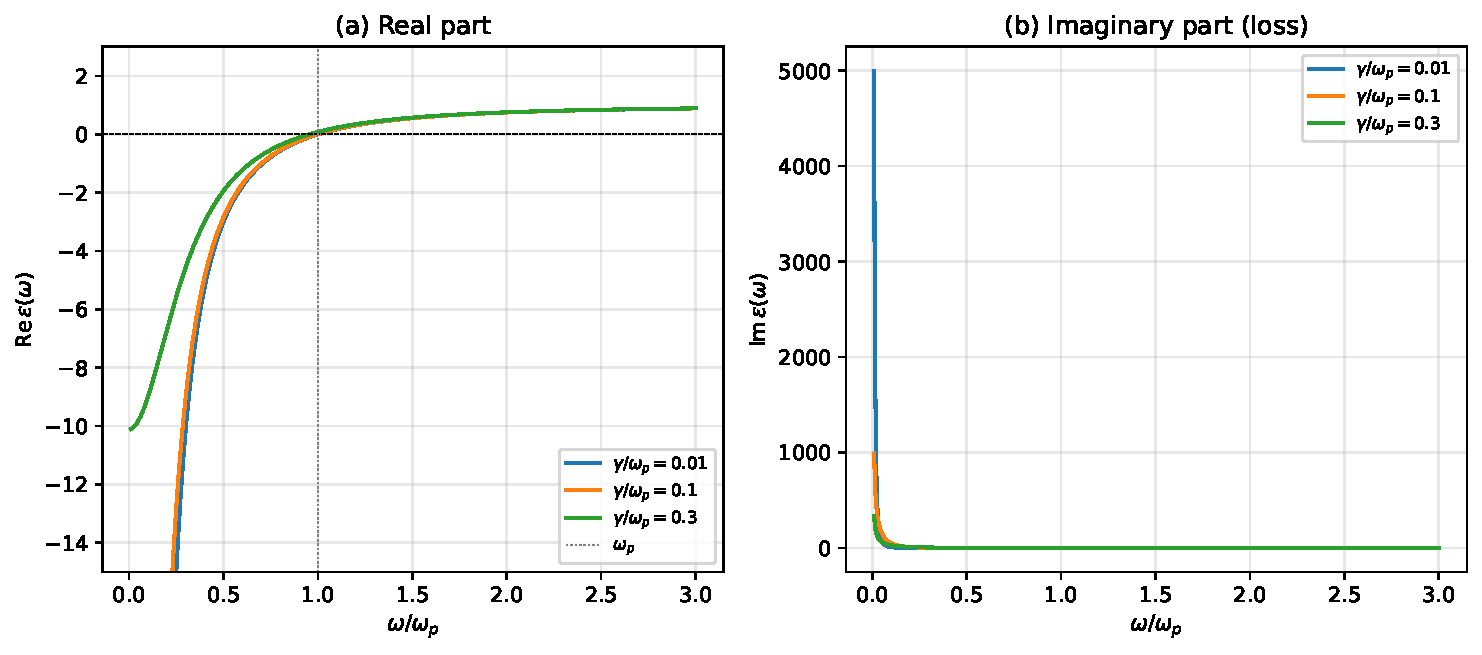
\includegraphics[width=0.85\linewidth]{figures/fig_f05_drude_permittivity.pdf}
 \caption{Drude permittivity for a free-electron metal.
 (a)~$\Re\,\varepsilon(\omega)$ is negative below the plasma frequency
 $\omega_p$ (vertical dotted line) and approaches $+1$ at high
 frequencies. Increasing the damping rate $\gamma$ smooths the
 divergence near $\omega = 0$.
 (b)~$\Im\,\varepsilon(\omega)$ is peaked at low frequencies where
 ohmic absorption dominates. The interplay of negative
 $\Re\,\varepsilon$ and finite $\Im\,\varepsilon$ is the origin of
 plasmonic resonances in metallic nanostructures.}
 \label{fig:drude-permittivity}
\end{figure}

\subsection{Passivity and the power dissipation condition}
\label{ssec:passivity}

A passive medium absorbs more energy than it emits at every frequency.
This imposes the \emph{power dissipation condition}:
\begin{equation}
 \omega\,\epsr''(\omega) \ge 0
 \qquad\text{for all real } \omega.
 \label{eq:passivity}
\end{equation}
For positive frequencies, this means $\epsr'' \ge 0$: absorption. For
an active (gain) medium, $\epsr'' < 0$ at some positive frequencies,
violating passivity. Gain media are driven out of thermodynamic
equilibrium by an external pump (optical or electrical), and the
Kramers--Kronig relations must be applied to the full response including
the pump-induced changes~\cite{figotin2004hamiltonian}.


%% ================================================================
\section{Energy in lossy and dispersive media}
\label{sec:dispersive-energy}

The time-averaged energy density~\eqref{eq:time-avg-u} was derived for
real, nondispersive $\epsr$. When $\epsr(\omega)$ is complex and
frequency-dependent, the energy stored in the medium is no longer given
by $\frac{1}{4}\epsvac\epsr|\EE|^2$.

\subsection{The Brillouin formula}
\label{ssec:brillouin}

For a lossless dispersive medium, or for a low-loss medium observed over a
transparent narrow band centered at frequency $\omega_0$, the
time-averaged energy density is approximately
\begin{equation}
 \langle u\rangle_{\mathrm{disp}}
 = \frac{1}{4}\epsvac\,
 \dv{}{\omega}\!\bigl[\omega\,\epsr'(\omega)\bigr]
 \bigg|_{\omega_0}\!\!|\EE|^2
 + \frac{1}{4}\muvac\,
 \dv{}{\omega}\!\bigl[\omega\,\mur'(\omega)\bigr]
 \bigg|_{\omega_0}\!\!|\HH|^2.
 \label{eq:brillouin-full}
\end{equation}
This is the \emph{Brillouin formula}, widely used in textbooks. It
reduces to the nondispersive result when $\epsr$ is constant.

However, the Brillouin formula has severe limitations:
\begin{enumerate}
 \item It assumes a transparent or weakly absorbing frequency window, so
 that a stored energy can be separated cleanly from irreversible heat.
 \item Near an absorption resonance, using only the real part of a
 lossy permittivity can give misleading or even negative apparent
 ``energy densities.''
 \item It accounts for material polarization energy only indirectly,
 through the frequency derivative of the constitutive parameters.
 \item It cannot be used as an inner product for mode
 orthogonality, because it depends on $\omega$ and is not bilinear.
\end{enumerate}

\subsection{Example: energy density near a Lorentz resonance}
\label{ssec:brillouin-lorentz}

For the single Lorentz oscillator~\eqref{eq:lorentz-eps} in the lossless
limit $\gamma\to 0$, the Brillouin energy factor is
\begin{equation}
 \dv{}{\omega}\bigl[\omega\,\epsr'(\omega)\bigr]
 = 1 + \omega_p^2\,
 \frac{\omega_0^2 + \omega^2}{(\omega_0^2-\omega^2)^2}.
 \label{eq:brillouin-lorentz}
\end{equation}
Away from resonance, this is positive and large, correctly capturing the
additional energy stored in the material polarization. At the resonance
itself the lossless formula
diverges, signaling that the transparent-medium approximation has broken
down. With finite damping, a meaningful energy balance must include the
oscillator and bath degrees of freedom explicitly; substituting only
$\epsr'(\omega)$ into the Brillouin formula is then no longer a reliable
inner product.

\subsection{Why a simple inner product fails}
\label{ssec:no-simple-inner}

The root of the difficulty is that the reduced macroscopic Maxwell
equations---written in terms of $\EE$ and $\HH$ alone---describe an
\emph{open subsystem}: the material degrees of freedom (atomic
oscillators, free carriers, phonons) have been integrated out, leaving
only their effect as a frequency-dependent $\epsr(\omega)$. The full
system (fields plus matter) conserves energy, but the reduced system does
not, because energy flows between the fields and the material oscillators.
Attempting to define a conserved energy for the fields alone is like
trying to define a conserved energy for one particle in a two-body
problem~\cite{figotin2004hamiltonian}.


%% ================================================================
\section{Auxiliary fields and the Hamiltonian embedding}
\label{sec:auxiliary-fields}

The resolution, developed rigorously by Figotin and
Schenker~\cite{figotin2004hamiltonian}, is to \emph{restore} the material
degrees of freedom as explicit auxiliary fields and construct a
conservative extended system.

\subsection{The idea}
\label{ssec:aux-idea}

Consider a medium whose susceptibility $\hat{\chi}(\omega)$ satisfies the
causality, passivity, and Kramers--Kronig conditions. The Lorentz model
\eqref{eq:lorentz-eps} can be written as
\begin{equation}
 \hat{\chi}(\omega)
 = \frac{\omega_p^2}{\omega_0^2 - \omega^2 - i\gamma\omega}
 = \int_0^\infty\!\frac{J(\nu)}{\nu^2 - \omega^2 - i\gamma'\omega}\;\dd\nu,
 \label{eq:spectral-representation}
\end{equation}
where the second form generalizes to any causal susceptibility via a
spectral representation (a continuous distribution of oscillator strengths
$J(\nu)$). Each oscillator mode at frequency $\nu$ is promoted to an
explicit dynamical variable---an auxiliary field $\mathbf{P}_\nu(\rr,t)$
that couples to $\EE$ and obeys its own equation of motion.

\subsection{Example: single Lorentz pole}
\label{ssec:aux-single-pole}

For a single Lorentz resonance, the auxiliary field is the polarization
density $\mathbf{P}(\rr,t)$. The coupled equations of motion are:
\begin{align}
 \epsvac\pdv{\EE}{t} &= \curl\HH - \pdv{\mathbf{P}}{t},
 \label{eq:aux-ampere}\\
 \muvac\pdv{\HH}{t} &= -\curl\EE,
 \label{eq:aux-faraday}\\
 \pdv[2]{\mathbf{P}}{t} + \gamma\pdv{\mathbf{P}}{t} + \omega_0^2\mathbf{P}
 &= \epsvac\omega_p^2\,\EE.
 \label{eq:aux-oscillator}
\end{align}
Equation~\eqref{eq:aux-oscillator} is the Lorentz oscillator equation.
Taking the Fourier transform and solving for $\mathbf{P}(\omega)$ gives
$\mathbf{P}(\omega) = \epsvac\hat{\chi}(\omega)\EE(\omega)$, recovering
the Lorentz permittivity~\eqref{eq:lorentz-eps}.

The damping term $\gamma\partial\mathbf{P}/\partial t$ is the source of
non-Hermiticity: it represents energy transfer from the coherent
polarization to an incoherent bath. Without it ($\gamma = 0$), the
system~\eqref{eq:aux-ampere}--\eqref{eq:aux-oscillator} is
conservative and can be written in Hamiltonian form.

\subsection{The extended Hamiltonian}
\label{ssec:extended-hamiltonian}

For $\gamma = 0$, define the canonical momentum of the polarization
oscillator as $\mathbf{Q} = \partial\mathbf{P}/\partial t$. The total
energy of the extended system is
\begin{equation}
 \mathcal{H} = \frac{1}{2}\int\!\left[
 \epsvac|\EE|^2 + \muvac|\HH|^2
 + \frac{|\mathbf{Q}|^2}{\epsvac\omega_p^2}
 + \frac{\omega_0^2|\mathbf{P}|^2}{\epsvac\omega_p^2}
 \right]\dd^3r,
 \label{eq:aux-energy}
\end{equation}
which is manifestly positive definite and conserved by the coupled
equations. The first-order form is
\begin{equation}
 i\,\pdv{}{t}
 \begin{pmatrix} \EE \\ \HH \\ \mathbf{P} \\ \mathbf{Q} \end{pmatrix}
 = \hat{\mathcal{H}}_{\mathrm{ext}}
 \begin{pmatrix} \EE \\ \HH \\ \mathbf{P} \\ \mathbf{Q} \end{pmatrix},
 \label{eq:extended-system}
\end{equation}
where $\hat{\mathcal{H}}_{\mathrm{ext}}$ is self-adjoint with respect to
the extended energy inner product~\eqref{eq:aux-energy}.

When the auxiliary fields are eliminated (by solving their equations of
motion in terms of $\EE$), one recovers the original reduced Maxwell
equations with the frequency-dependent $\epsr(\omega)$. But in the
reduced system, the total energy is no longer conserved: some of it has
been transferred to the hidden oscillators.

For $\gamma > 0$, the damping term breaks the Hermiticity of
$\hat{\mathcal{H}}_{\mathrm{ext}}$. The extended system is then
non-conservative, and a further embedding into a larger Hilbert space
(a Lindblad or Caldeira--Leggett bath) is needed for a fully Hamiltonian
treatment~\cite{figotin2004hamiltonian}.

\begin{takeaway}[Non-Hermiticity from elimination]
The macroscopic Maxwell equations with frequency-dependent $\epsr(\omega)$
are non-Hermitian not because the physics is non-conservative, but because
the conservative degrees of freedom of the material have been eliminated.
Restoring them through auxiliary fields recovers a Hamiltonian (Hermitian)
description of the full system. This is the third road to non-Hermiticity
identified in Chapter~\ref{ch:energy-inner}: not material loss, not
radiation, but frequency dispersion caused by eliminating material
variables from the Maxwell state.
\end{takeaway}


%% ================================================================
\section{Gain media}
\label{sec:gain-media}

An active (gain) medium has $\epsr''(\omega) < 0$ at frequencies within
the gain bandwidth. Physically, this requires an external energy source
(a pump) that maintains a population inversion or stimulated emission
process.

\subsection{The inverted Lorentz model}
\label{ssec:inverted-lorentz}

The Lorentz oscillator model can be adapted to describe gain by reversing
the sign of the damping: $\gamma \to -|\gamma|$. As a small-signal
phenomenological model near a pumped transition, this gives
\begin{equation}
 \varepsilon_{\mathrm{gain}}(\omega)
 = 1 + \frac{\omega_p^2}
 {\omega_0^2 - \omega^2 + i|\gamma|\omega},
 \label{eq:gain-eps}
\end{equation}
with $\epsr'' < 0$ near $\omega_0$. The medium now amplifies rather than
absorbs. Taken literally over all frequencies, negative damping would be
an unstable linear oscillator; in a real gain medium the pump, finite
bandwidth, and saturation nonlinearity regularize the response.

\subsection{Population inversion and the four-level system}
\label{ssec:population-inversion}

In a real laser medium, gain arises from population inversion between
two electronic levels. The simplest tractable model is the four-level
system with levels $|0\rangle$, $|1\rangle$, $|2\rangle$, $|3\rangle$:
an external pump excites atoms from $|0\rangle$ to $|3\rangle$; rapid
non-radiative decay brings atoms from $|3\rangle$ to $|2\rangle$ (the
upper laser level); stimulated emission occurs on the
$|2\rangle \to |1\rangle$ transition, providing gain at the lasing
frequency $\omega_L = (E_2 - E_1)/\hbar$; and rapid decay from
$|1\rangle$ to $|0\rangle$ empties the lower laser level, maintaining
inversion.

The gain coefficient is proportional to the population difference
$\Delta N = N_2 - N_1 > 0$ and to the transition cross section
$\sigma(\omega)$:
\begin{equation}
 g(\omega) = \sigma(\omega)\,\Delta N,
 \label{eq:gain-coefficient}
\end{equation}
where $\sigma(\omega)$ has a Lorentzian line shape centered at $\omega_L$.
The imaginary permittivity contributed by the gain transition is
$\epsr''(\omega) = -cn\, g(\omega)/\omega < 0$.

\paragraph{Rate equations for the four-level system.}
The steady-state populations are governed by the rate equations.
Because the relaxation rates $\gamma_{32}$ (from $|3\rangle$ to
$|2\rangle$) and $\gamma_{10}$ (from $|1\rangle$ to $|0\rangle$) are
fast, the populations $N_3$ and $N_1$ are approximately zero in steady
state, and the total population satisfies $N_0 + N_2 \approx N_{\mathrm{tot}}$.
The rate equation for the upper laser level is
\begin{equation}
 \dv{N_2}{t} = R_{\mathrm{pump}} - \frac{\sigma(\omega_L)\,I}{\hbar\omega_L}\,\Delta N
 - \frac{N_2}{\tau_{\mathrm{sp}}} = 0,
 \label{eq:rate-equation-n2}
\end{equation}
where $R_{\mathrm{pump}}$ is the pump rate (atoms per unit volume per
unit time), $I$ is the intracavity intensity, $\tau_{\mathrm{sp}}$ is
the spontaneous emission lifetime of the upper level, and the middle
term represents the stimulated emission rate. Since
$N_1 \approx 0$, we have $\Delta N \approx N_2$.

Solving~\eqref{eq:rate-equation-n2} for $N_2$ in steady state:
\begin{equation}
 N_2 = \frac{R_{\mathrm{pump}}\,\tau_{\mathrm{sp}}}
 {1 + I/I_{\mathrm{sat}}},
 \qquad
 I_{\mathrm{sat}} = \frac{\hbar\omega_L}{\sigma(\omega_L)\,\tau_{\mathrm{sp}}},
 \label{eq:saturation-derivation}
\end{equation}
where we identify the small-signal inversion
$\Delta N_0 = R_{\mathrm{pump}}\,\tau_{\mathrm{sp}}$ (the inversion in
the absence of stimulated emission). Substituting into
Eq.~\eqref{eq:gain-coefficient} immediately recovers the saturated gain
formula~\eqref{eq:gain-saturation}:
\begin{equation}
 g(I) = \sigma\,\Delta N_0 \cdot \frac{1}{1 + I/I_{\mathrm{sat}}}
 = \frac{g_0}{1 + I/I_{\mathrm{sat}}}.
 \label{eq:gain-saturation-derived}
\end{equation}
The saturation intensity $I_{\mathrm{sat}}$ has a transparent physical
meaning: it is the intensity at which the stimulated emission rate
$\sigma I/(\hbar\omega_L)$ equals the spontaneous decay rate
$1/\tau_{\mathrm{sp}}$. Below this intensity, stimulated emission is a
small perturbation on the inversion; above it, stimulated emission
dominates and the gain is depleted.

\paragraph{Gain clamping and threshold.}
At steady-state lasing, the gain must exactly compensate the total cavity
loss $\alpha_{\mathrm{tot}}$ (including mirror loss and material
absorption):
\begin{equation}
 g(I_{\mathrm{ss}}) = \alpha_{\mathrm{tot}} \quad\Rightarrow\quad
 I_{\mathrm{ss}} = I_{\mathrm{sat}}\left(\frac{g_0}{\alpha_{\mathrm{tot}}} - 1\right).
 \label{eq:gain-clamping}
\end{equation}
This is the gain-clamping condition. Below threshold
($g_0 < \alpha_{\mathrm{tot}}$), no steady-state lasing occurs and
$I_{\mathrm{ss}} = 0$. Above threshold, the intracavity intensity
grows linearly with pump power (since $g_0 \propto R_{\mathrm{pump}}$),
while the material gain clamps at $\alpha_{\mathrm{tot}}$---it cannot
exceed the loss, because any excess gain would increase $I$, which would
further deplete the inversion until balance is restored.

\paragraph{Connection to the Maxwell framework.}
The gain-clamping condition connects the microscopic rate equations to
the macroscopic Maxwell eigenproblem. The intensity-dependent
permittivity of the gain medium is
\begin{equation}
 \epsr(\omega, I) = \epsr'(\omega)
 - i\,\frac{c\,n_{\mathrm{bg}}\,g(I)}{\omega}
 = \epsr'(\omega)
 - i\,\frac{c\,n_{\mathrm{bg}}\,g_0}{\omega(1 + I/I_{\mathrm{sat}})},
 \label{eq:eps-saturated}
\end{equation}
where $n_{\mathrm{bg}}$ is the background refractive index and the
negative sign of the imaginary part reflects gain (with our
$e^{-i\omega t}$ convention, $\epsr'' < 0$ corresponds to
amplification). This intensity-dependent permittivity makes the
Maxwell eigenproblem nonlinear: the eigenfrequencies depend on the
field amplitudes through $I$. The linear non-Hermitian framework
of this book treats $\epsr$ as independent of $I$---an approximation
valid below or near threshold, where $I \ll I_{\mathrm{sat}}$ and
$g \approx g_0$. Above threshold, the full nonlinear problem must
be solved self-consistently, as discussed in
Chapter~\ref{ch:open-problems}.

\subsection{Gain saturation}
\label{ssec:gain-saturation}

As the intracavity field intensity $I$ grows, stimulated emission depletes
the population inversion. The saturated gain coefficient is
\begin{equation}
 g(I) = \frac{g_0}{1 + I/I_{\mathrm{sat}}},
 \label{eq:gain-saturation}
\end{equation}
where $g_0$ is the small-signal gain and $I_{\mathrm{sat}}$ is the
saturation intensity. At threshold, the saturated gain equals the total
loss. Above threshold, the gain clamps at the loss value, and additional
pump power is converted into laser output power.

\begin{figure}[t]
 \centering
 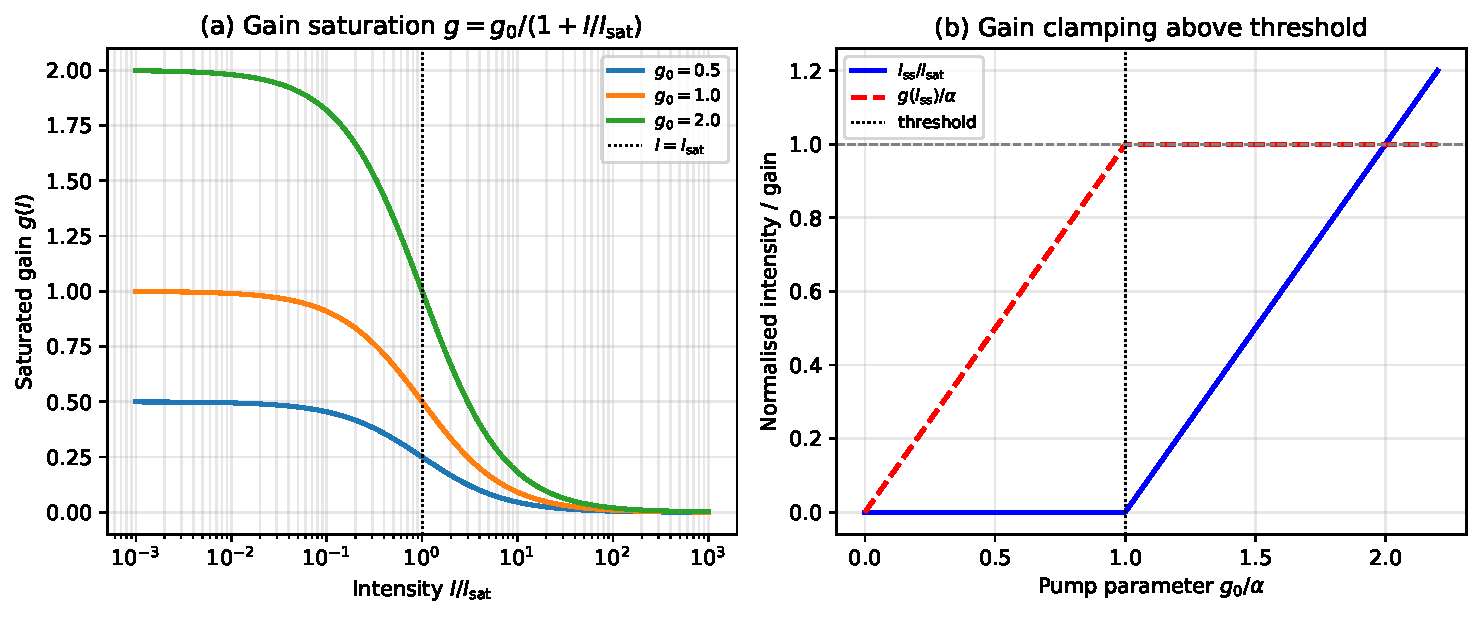
\includegraphics[width=0.85\linewidth]{figures/fig_f05_gain_saturation_rate.pdf}
 \caption{Gain saturation and gain clamping in a four-level laser model.
 (a)~The saturated gain $g(I)=g_0/(1+I/I_{\mathrm{sat}})$ decreases once
 the intracavity intensity becomes comparable with the saturation
 intensity $I_{\mathrm{sat}}$. (b)~Above threshold, the steady-state
 intensity grows as $I_{\mathrm{ss}}/I_{\mathrm{sat}}=g_0/\alpha-1$
 while the material gain clamps to the total loss $\alpha$. This is the
 nonlinear mechanism that prevents the linear gain model from producing
 unbounded fields above threshold.}
 \label{fig:gain-saturation-rate}
\end{figure}


Gain saturation is intrinsically nonlinear: the permittivity depends on
the field amplitude. The linear non-Hermitian framework developed in
this book is therefore strictly valid only below or near the lasing
threshold. Above threshold, the coupling between the gain medium and the
cavity field requires a nonlinear analysis
(Chapter~\ref{ch:open-problems}).

\paragraph{Quantitative example: InGaAsP gain medium.}
For a typical InGaAsP multiple-quantum-well gain medium~\cite{huang2023resonant,koshelev2018nonradiating} at
$\lambda = 1550\;$nm, the small-signal material gain coefficient is
$g_0 \approx 400\;$cm$^{-1}$ at a carrier density
$N = 3 \times 10^{18}\;$cm$^{-3}$, and the saturation intensity is
$I_{\mathrm{sat}} \approx 5 \times 10^{8}\;$W/m$^2$ (corresponding to
a saturation photon density
$n_{\mathrm{ph,sat}} \approx 2.6 \times 10^{15}\;$cm$^{-3}$).
The corresponding imaginary permittivity is
$\varepsilon'' = -cn g_0/\omega \approx -0.031$ at small signal.
For a photonic crystal cavity with mode volume
$V_{\mathrm{mode}} \sim (\lambda/n)^3 \approx 0.05\;\mu$m$^3$ and
$\Qfac = 5000$, the threshold condition
$g_{\mathrm{th}} = \omega/(c\,\Qfac) \approx 40\;$cm$^{-1}$ is reached
at a pump current of roughly $50\;\mu$A---well within the linear regime
where $g/g_0 \approx 0.1$ and saturation corrections are small. As the
pump increases toward $g_0$, the saturation nonlinearity becomes
important and the linear non-Hermitian description begins to break down.

\begin{figure}[t]
 \centering
 
\includegraphics[width=0.96\linewidth]{fig_f5_gain_saturation.pdf}
 \caption{Gain saturation in a homogeneous medium.
 (a)~Normalized gain $g(I)/g_0 = 1/(1+I/I_{\mathrm{sat}})$ versus
 intensity. The half-gain point occurs at $I = I_{\mathrm{sat}}$.
 (b)~Normalized $|\varepsilon''|/|\varepsilon''_0|$ (solid red) and
 $g/g_0$ (dashed green) plotted on the same vertical scale, confirming
 that both quantities share the same saturation dependence; the
 conversion is $|\varepsilon''| = c\,n\,g/\omega$. Parameters:
 $g_0 = 400\;\mathrm{cm}^{-1}$,
 $\varepsilon''_0 \approx -0.031$,
 $\lambda = 1550\;\mathrm{nm}$,
 $n_{\mathrm{eff}} = 3.4$.}
 \label{fig:gain-saturation}
\end{figure}

\paragraph{Kramers--Kronig constraints on gain media.}
A gain medium with $\varepsilon''(\omega) < 0$ over a spectral band~\cite{rter2010observation,feng2012experimental}
must, by the Kramers--Kronig relations, also exhibit anomalous
dispersion $\dd\varepsilon'/\dd\omega < 0$ within the same band. This
is because the subtracted dispersion relation
$\varepsilon'(\omega) - \varepsilon'(\infty) =
(2/\pi)\,\mathcal{P}\!\int_0^\infty
\omega'\varepsilon''(\omega')/(\omega'^2-\omega^2)\;\dd\omega'$
has the same structure for gain as for loss, with reversed sign of
$\varepsilon''$. The anomalous dispersion in the gain band reduces the
group velocity and can even make it superluminal or negative, though the
signal velocity remains bounded by $c$ because the gain bandwidth is
always finite. This connection between gain and anomalous dispersion is
important for understanding the frequency-pulling effect in lasers and
the bandwidth limitations of optical amplifiers.


%% ================================================================
\section{Balanced gain and loss: the $\PT$-symmetric condition}
\label{sec:pt-preview}

A medium with spatial regions of loss and gain, arranged so that
\begin{equation}
 \epsr(\rr) = \epsr^*(-\rr),
 \label{eq:pt-condition-preview}
\end{equation}
has a special symmetry: $\PT$ symmetry. The real part of $\epsr$ is
symmetric and the imaginary part is antisymmetric under spatial inversion.
This condition ensures that the total gain and loss are balanced, and the
system can exhibit a phase transition from real to complex eigenfrequencies.
The physics of $\PT$-symmetric optical systems is the subject of
Chapter~\ref{ch:pt-symmetric}.

\subsection{The $\PT$-symmetric Lorentz model}
\label{ssec:pt-lorentz}

A one-dimensional $\PT$-symmetric refractive-index profile can be
constructed from two Lorentz media with opposite signs of damping:
\begin{equation}
 \epsr(x,\omega) = \begin{cases}
 \eps_{\mathrm{bg}} + \Delta\eps_{\mathrm{Lorentz}}(\omega;\gamma) & x > 0,\\
 \eps_{\mathrm{bg}} + \Delta\eps_{\mathrm{Lorentz}}(\omega;-\gamma) & x < 0,
 \end{cases}
 \label{eq:pt-lorentz-profile}
\end{equation}
where $\gamma > 0$ and $\eps_{\mathrm{bg}}$ is real. This satisfies
$\epsr(x,\omega)=\epsr^*(-x,\omega)$ on the real-frequency axis and provides a
microscopically motivated realization of the $\PT$ condition for the
transfer-matrix and coupled-mode analyses of
Chapter~\ref{ch:pt-symmetric}.


%% ================================================================
\section{Summary and connections}
\label{sec:ch5-forward}

Material loss, gain, and dispersion---the first road to
non-Hermiticity---are not ad hoc modifications of Maxwell's
equations but an inevitable consequence of the causal, dissipative
response of real materials:

\begin{itemize}
 \item Linear response and causality require $\epsr(\omega)$ to be
 complex and frequency-dependent, constrained by the
 Kramers--Kronig relations and sum rules.
 \item The imaginary part $\epsr''$ breaks the self-adjointness of the
 Maxwell operator by making the constitutive weight complex and by
 allowing irreversible exchange of energy with the material.
 \item The Brillouin formula provides a useful but limited
 approximation to the energy in dispersive media; a rigorous
 treatment requires auxiliary fields and an extended Hamiltonian.
 \item Gain media violate passivity through population inversion and
 can lead to lasing when coupled with feedback; gain saturation
 makes the linear non-Hermitian description valid only near or
 below threshold.
 \item The special case of balanced gain and loss ($\PT$ symmetry)
 connects to a rich phenomenology explored in
 Chapter~\ref{ch:pt-symmetric}.
\end{itemize}

Several threads connect forward from this material foundation:
\begin{enumerate}
 \item The complex QNM frequencies of Chapter~\ref{ch:qnm} arise from
 material loss ($\varepsilon'' > 0$) combined with radiative loss
 from open boundaries.
 \item The $\PT$-symmetric condition
 $\varepsilon(\rr) = \varepsilon^*(-\rr)$ of
 Chapter~\ref{ch:pt-symmetric} is a precise spatial arrangement of
 the gain and loss physics developed here.
 \item The dispersive auxiliary-field formulation of
 Section~\ref{sec:auxiliary-fields} reappears in
 Chapter~\ref{ch:numerics} as the basis for finite-element
 eigensolvers that handle frequency-dependent materials without
 nonlinear eigenvalue problems.
 \item Gain saturation provides the nonlinear feedback that stabilises
 lasers and creates the nonlinear exceptional points discussed in
 Chapters~\ref{ch:pt-symmetric} and~\ref{ch:open-problems}.
 \item The Kramers--Kronig constraint that gain media must exhibit
 anomalous dispersion limits the bandwidth of optical amplifiers and
 modifies the group velocity of pulses propagating through active
 photonic structures.
\end{enumerate}

Chapter~\ref{ch:qnm} now turns to the second physical origin of
non-Hermiticity---radiation and openness---and develops the quasinormal-mode
theory that provides the natural eigenstates of the non-self-adjoint
Maxwell operator.

\begin{takeaway}[Material non-Hermiticity is physical, not mathematical]
Complex permittivity, frequency dispersion, gain saturation, and
auxiliary-field embeddings are not formal devices introduced for
mathematical convenience. They encode the irreversible exchange of
energy between the electromagnetic field and matter---absorption heating,
stimulated emission, and the frequency-dependent phase response of bound
electrons. Every non-Hermitian photonic phenomenon studied in the
remainder of this book has its material origin in the physics of this
chapter.
\end{takeaway}
